\subsubsectionlink{デコヒーレンスの漸進的作用を観測する}
最初の原子の通過と測定は、その状態に関する情報を共振器Cへ残すことに注意しよう。測定結果に応じて、C内の場の最終状態が、$|\psi_{\mathrm{field}}^{(g)}\rangle$または$|\psi_{\mathrm{field}}^{(e)}\rangle$となるからである。(6.18)、(6.19)から分かるように、この情報は、重ね合わせの成分$|\alpha\rangle$と$|-\alpha\rangle$の相対符号に符号化されている。デコヒーレンスは、このような位相情報を環境へ非局在化し、系の水準では利用できなくする傾向があることを知っている。その結果としてのコヒーレンスの減衰を、どう監視できるだろうか。

その仕掛けは、探針として働く第二の原子を、共振器列$R_1\to\mathrm C\to R_2$へ送ることである。第一の原子の通過後、十分速くこれを行えば、第一の原子についての情報は、共振器Cの場の状態へまだよく符号化されており、第二の原子はこの情報と相関する。注目すべき結果は、デコヒーレンスがなく、光子数が$\bar n=|\alpha|^2\gg1$なら、$D_e$または$D_g$での検出後、第二の原子は常に第一の原子と同じ状態に見いだされることである。

実際にそうなることは、次の簡単な計算から容易に分かる（図6.3参照）。原子1が$|e\rangle$状態で検出され、場の状態が$|\psi_{\mathrm{field}}^{(e)}\rangle$となったと仮定しよう。共振器$R_1$を通過した原子2は、重ね合わせ$|\psi_{\mathrm{atom2}}\rangle=(|g\rangle+|e\rangle)/\sqrt2$［(6.10)参照］で記述される。ここでは、基底状態$|g\rangle$と$|e\rangle$は原子2を指す。したがって、この原子と場の、初めの無相関な状態は、
\begin{equation}|\Psi_{\mathrm{atom2+field}}\rangle=\frac12(|g\rangle+|e\rangle)(-|\alpha\rangle+|-\alpha\rangle).\tag{6.20}\end{equation}
原子2が共振器Cを通ると何が起きるだろうか。原子が$|e\rangle$状態なら、場の状態は位相シフト$|\pm\alpha\rangle\to|\mp\alpha\rangle$を受けることを思い出そう。したがって、Cを通過した後の結合状態は、
% 原文 p.252
\hypertarget{srcpage:252}{}\label{srcpage:252}
\begin{equation}|\Psi_{\mathrm{atom2+field}}\rangle=\frac12(-|g\rangle|\alpha\rangle+|g\rangle|-\alpha\rangle-|e\rangle|-\alpha\rangle+|e\rangle|\alpha\rangle).\tag{6.21}\end{equation}
となる。次に原子は共振器$R_2$を通過し、$|g\rangle$と$|e\rangle$がこれらの状態の重ね合わせへ変換される［(6.16)参照］。したがって状態(6.21)は、
\begin{equation}\begin{aligned}
|\Psi_{\mathrm{atom2+field}}\rangle
&=\frac1{2\sqrt2}\bigl(-|g\rangle|\alpha\rangle+|e\rangle|\alpha\rangle+|g\rangle|-\alpha\rangle-|e\rangle|-\alpha\rangle\\
&\qquad-|e\rangle|-\alpha\rangle-|g\rangle|-\alpha\rangle+|e\rangle|\alpha\rangle+|g\rangle|\alpha\rangle\bigr)\\
&=\frac1{\sqrt2}|e\rangle(|\alpha\rangle-|-\alpha\rangle).
\end{aligned}\tag{6.22}\end{equation}
となる。$|\alpha\rangle$と$|-\alpha\rangle$が直交すると仮定すれば、共振器C内の光子数$\bar n=|\alpha|^2$が増すほどよい近似となるが、状態(6.22)に対応する原子2の縮約密度演算子は、
\begin{equation}
\hat\rho_{\mathrm{atom2}}=\operatorname{Tr}_{\mathrm{field}}|\Psi_{\mathrm{atom2+field}}\rangle\langle\Psi_{\mathrm{atom2+field}}|=|e_2\rangle\langle e_2|.\tag{6.23}
\end{equation}
直ちに、原子1が$|e\rangle$状態で検出されたとき、原子2を$|e\rangle$状態に見いだす確率$P_{ee}$は、$P_{ee}=1$となる。
% 原文 p.253
\hypertarget{srcpage:253}{}\label{srcpage:253}
原子1が$|g\rangle$状態で検出されたという仮定の下でも、同様の計算ができる。これで、二原子の完全な相関についての、上の主張が確立された。

\begin{figure}[htbp]\centering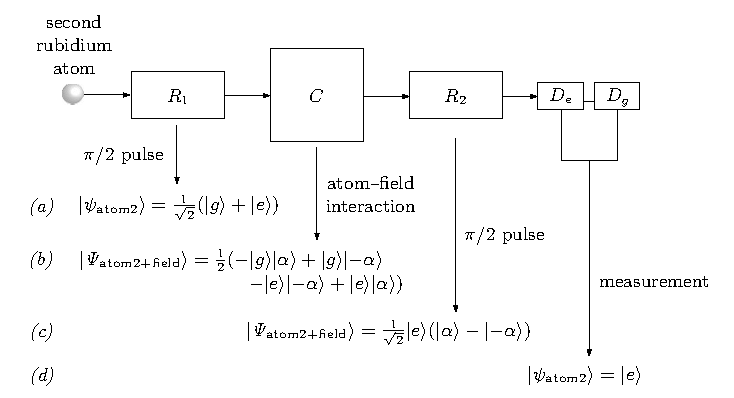
\includegraphics[width=.96\linewidth]{figures/ch06_fig03.pdf}
\caption{第一の原子が$|e\rangle$状態で検出されたと仮定したとき、共振器C内の場の重ね合わせ状態を検出し、そのデコヒーレンスを監視する事象の系列。(a)共振器$R_1$の$\pi/2$パルスが、第二のRb原子を$|g\rangle$、$|e\rangle$の重ね合わせ(6.20)に準備する。(b)原子は、第一の原子の通過後、重ね合わせ状態に残された共振器Cへ入る。原子2はC内の場へ別の位相シフトを与え、もつれた原子・場状態［(6.21)参照］を作る。(c)共振器$R_2$の$\pi/2$パルスが、場と原子のもつれを解く［(6.22)参照］。(d)場の状態$|\pm\alpha\rangle$が近似的に直交するなら、原子2は常に、原子1と同じ$|e\rangle$状態で検出される。したがって、二つの測定結果は完全に相関する。この相関の減衰は、共振器Cの猫状態のデコヒーレンスを意味する。}
\end{figure}

ゆえに、猫状態のデコヒーレンスを観測するために必要なのは、第一、第二の原子を送り出す時間間隔$T$を増やしながら、原子対の測定結果間の相関$P_{ee}(T)$、あるいは$P_{gg}(T)$の減衰を測定することだけである。$T$が場の重ね合わせの特徴的なデコヒーレンス時間よりはるかに小さければ、$P_{ee}(T)$は1に近くなる。重ね合わせがまだほとんどデコヒーレンスしていないときの、測定結果間の完全な相関を反映するのである。遅延時間$T$を長くすると、共振器内の重ね合わせは、ますますデコヒーレンスする。やがて、すべての相対位相情報、したがって第一の原子の状態の情報が環境へ非局在化し、場は非コヒーレントな統計的混合
\begin{equation}\hat\rho_{\mathrm{field}}=\frac12(|\alpha\rangle\langle\alpha|+|-\alpha\rangle\langle-\alpha|)\tag{6.24}\end{equation}
で記述される。このとき、第一、第二の原子の測定結果は完全に無相関となる。すなわち、第二の原子の測定結果はランダムであり、第一の原子の測定結果から独立になる。したがって、このデコヒーレンス過程は、$P_{ee}(T)$が$1/2$まで減衰することとして観測できる。

図6.4は、$P_{ee}(T)$の理論予測\cite{ref250}を示し、これは実験観測\cite{ref251}と非常によく一致した。$P_{ee}(T)$が初期値1からかなり急速に低下し、完全なデコヒーレンスに対応する$P_{ee}(T)=1/2$の平坦部に達する様子が明瞭に見える。読者は、$P_{ee}(T)$がある範囲の遅延時間$T$にわたり$1/2$付近にとどまった後、より大きい$T$で、なぜ突然また0へ向かって減衰するのかと、疑問に思うかもしれない。説明は非常に簡単である。共振器C内の光子寿命は有限なので、やがてC内に光子がなくなる。すると、Cを通過する原子に対する効果はなくなる。この場合、原子が受けるのは、共振器$R_1$と$R_2$の二つの$\pi/2$パルスだけであり、それらの合成効果は、初期状態$|e\rangle$を$|g\rangle$へ変換することである［(6.16)参照］。
\begin{equation}|e\rangle\xrightarrow{\pi/2}\frac1{\sqrt2}(|g\rangle+|e\rangle)\tag{6.25}\end{equation}
\begin{equation}\xrightarrow{\pi/2}\frac1{\sqrt2}\left[\frac1{\sqrt2}(|g\rangle-|e\rangle)+\frac1{\sqrt2}(|g\rangle+|e\rangle)\right]=|g\rangle.\tag{6.26}\end{equation}
したがって、原子は決して$|e\rangle$状態で検出されず、$T\to\infty$で$P_{ee}(T)\to0$となる。

図6.4のグラフから、場の重ね合わせの特徴的デコヒーレンス時間を読み取れる。実験では、それが二つの主要パラメーターに依存することが示された。
% 原文 p.254
\hypertarget{srcpage:254}{}\label{srcpage:254}
\begin{figure}[htbp]\centering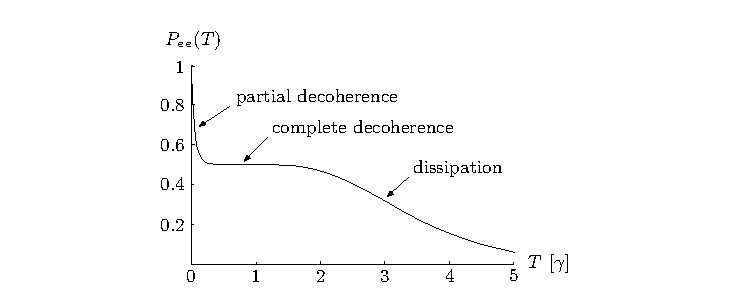
\includegraphics[width=.85\linewidth]{figures/ch06_fig04.pdf}
\caption{Davidovichら\cite{ref250}による、一対の原子が通過する遅延時間$T$への、同時確率$P_{ee}(T)$の依存性。初期の速い減衰は、共振器Cの猫状態のデコヒーレンスに対応し、$P_{ee}(T)=1/2$は完全なデコヒーレンスを表す。さらに大きな$T$では、共振器からの光子漏出によって$P_{ee}(T)$がさらに低下する。遅延時間$T$の単位は、共振器の特徴的散逸期間$\gamma$である。許可を得て\cite{ref250}の図を改作。Copyright 1996 by the American Physical Society.}
\end{figure}
\begin{enumerate}
\item 共振器Cを通過する$|e\rangle$状態の原子が、場へ誘起する位相シフト$\varphi$。$\varphi$が大きいほど、場の重ね合わせのデコヒーレンス時間が短いことが分かった。これはもっともである。重ね合わせ状態の「猫らしさ」は、各成分をどれほど識別できるかに依存する。$\varphi$が小さければ、場の状態$|\alpha\rangle$と$|e^{i\varphi}\alpha\rangle$［(6.14)参照］の重なりは大きい。他方、$\varphi$が最大値$\pi$へ近づくと、これは上の議論で仮定した値であり、実験で達成した位相シフトにも近いが、二状態は直交し、したがって最大限に区別される。
\item 共振器C内の平均光子数$\bar n=|\alpha|^2$。これも理にかなっている。光子が多いほど、状態$|\Psi_{\mathrm{field}}^{(g,e)}\rangle$［(6.18)参照］は、より中間的尺度のもの、最終的には巨視的なものとなり、したがって、より強くデコヒーレンスを受ける。また、与えられた位相シフト$\varphi$について、$\bar n$が大きいほど成分$|\alpha\rangle$と$|e^{i\varphi}\alpha\rangle$の重なりは小さくなり、より区別される。
\end{enumerate}
Bruneたちは実験でこれらのパラメーターを変え、デコヒーレンス率がそれに応じて変わる様子を観測した。注目すべきことに、結果はDavidovichら\cite{ref250}の理論予測と驚くほどよく一致した。中間的尺度の「Schrödingerの子猫」を生成し、存在を検証し、そのデコヒーレンスを制御された仕方で観測したのは、これが初めてであった。

% 原文 p.255
\hypertarget{srcpage:255}{}\label{srcpage:255}
Bruneたちが行った型の実験は、その後、さらに多くの実験を生み、上述の結果が確認され、拡張されてきた。たとえば、共振器CのQ値を改善する必要があるが、その光子数を増すことで、ますます大きな猫状態を作れる。最近の実験では、数十個の光子が使われている\cite{ref252}。この種の実験は一般に「共振器量子電気力学」、略して「共振器QED」と呼ばれる。Schrödingerの猫状態の生成と、そのデコヒーレンスの観測だけでなく、共振器QEDは、量子コンピューターの実現にも使える可能性がある。さらに学びたい読者には、Dutraの本\cite{ref253}が、よい、しかも楽しく読める入門となる。

\subsubsectionlink{Schrödingerの猫を生き返らせる}
デコヒーレンスが完全にユニタリーで、したがって原理的に可逆な過程であるにもかかわらず、私たちは量子から古典への移行を「一方通行」と考えがちである。量子コヒーレンスが失われると、物体は古典的に振る舞い、量子世界へ戻すものは何もないように見える。もちろん、2.7節のデコヒーレンスの一般的議論から、それがあらゆる実用的目的について不可逆とみなされる理由を知っている。系の水準へ重ね合わせを実際に「再局在化」する、すなわちデコヒーレンス過程を実効的に時間反転するには、環境を適切に制御しなければならず、それは通常、実際には不可能だからである。

2.13節では、完全に制御できるよう適切に設計した「人工的」環境と系を相互作用させることで、仮想的デコヒーレンスの一例である、真に可逆なデコヒーレンス過程を調べられることを指摘した。1997年、Bruneのグループ\cite{ref254}は、前の各節の共振器QED実験を修正し、そのような設計された環境を含める案を提案した。2007年現在、この提案はまだ実験的に実現されていない。主な理由は、二つの超伝導共振器の間の可逆的結合が必要で、それを実際に実現するのが難しいからである。それでも、実験の考え方は非常に興味深く、技術的障害が近い将来に克服される見込みも高いため、本節で提案を概説する。

実験配置は、基本的に前述のものと同じである（図6.2参照）。主要な違いは、超伝導共振器Cを、たとえば超伝導導波路を用いて、初め空の、第二の同一共振器$\mathrm C_2$へ線形結合することである。追加の$\mathrm C_2$と明瞭に区別するため、以下では最初の共振器Cを$\mathrm C_1$と呼ぶ。この結合によって、$\mathrm C_1$と$\mathrm C_2$はエネルギー、すなわち光子を交換できる。Rb原子が装置を通過し、その状態が$D_e$、$D_g$で測定された後、共振器$\mathrm C_1$は二つの場の状態$|\alpha\rangle$、$|-\alpha\rangle$の重ね合わせに残されること［(6.18)、(6.19)参照］、
% 原文 p.256
\hypertarget{srcpage:256}{}\label{srcpage:256}
そして、二成分の相対符号が、測定された原子状態の情報を符号化することを思い出そう。

二共振器の結合によって、この位相情報が「貯蔵庫」$\mathrm C_2$へ移ったとする。このとき$\mathrm C_1$の状態は、対応して混合(6.24)で記述されなければならない。提案の考え方は、$\mathrm C_1$と$\mathrm C_2$の結合が十分高い程度まで可逆なら、その後この情報伝達の向きを逆転し、$\mathrm C_1$の初期重ね合わせを回復するとともに、$\mathrm C_2$を初期の空の状態へ戻せる、というものである。こうして、$\mathrm C_2$が$\mathrm C_1$に対する制御可能な単一モード環境として働き、$\mathrm C_1$のSchrödingerの猫状態をデコヒーレンスさせ、その後再出現させる、可逆なデコヒーレンス過程を模擬できる。

この議論をもう少し精密にしよう。二共振器間で、エネルギーが周波数$\Omega_{\mathrm C}$で振動的に交換されるとする。この周波数は、$\mathrm C_1$の猫状態の準備時間が、エネルギー交換の一周期よりはるかに短くなるよう選ぶ。したがって、二共振器の結合は重ね合わせ状態の準備に影響しないと仮定する。結合は線形なので、$\mathrm C_1$のコヒーレント場$|\alpha(t)\rangle$は、$\mathrm C_2$に別のコヒーレント場$|\beta(t)\rangle$を生じさせる。$t=0$で$\mathrm C_2$が場を含まないことを考慮すると、$\alpha(t)=\alpha_0\cos(\Omega_{\mathrm C}t/2)$、$\beta(t)=\alpha_0\sin(\Omega_{\mathrm C}t/2)$と書ける。したがって、$\mathrm C_1$の初期猫状態［(6.18)、(6.19)参照］
\begin{equation}|\Psi_{\mathrm C_1}^{(g,e)}\rangle=\frac1{\mathcal N}(\pm|\alpha\rangle+|-\alpha\rangle)\tag{6.27}\end{equation}
は、結合系$\mathrm C_1+\mathrm C_2$のもつれた状態へ発展する。
\begin{equation}|\Psi_{\mathrm C_1+\mathrm C_2}^{(g,e)}\rangle=\frac1{\mathcal N}(\pm|\alpha(t)\rangle|\beta(t)\rangle+|-\alpha(t)\rangle|-\beta(t)\rangle).\tag{6.28}\end{equation}
その後の振る舞いは、二つのコヒーレント場状態$|\pm\alpha\rangle$の重なりが、平均光子数$\bar n=|\alpha|^2$が増すほど減少することから、容易に理解できる。時間$t=\pi/\Omega_{\mathrm C}$後には$\beta(t)=\alpha_0$となり、すべての光子が$\mathrm C_2$に集中する。したがって$|\pm\beta\rangle$は最大限に区別され、$|\pm\alpha\rangle$の識別可能性は最小になる。これは、重ね合わせ成分の相対符号についての情報を、$\mathrm C_1$の犠牲の下で、$\mathrm C_2$が最大限保持することを意味する。言い換えれば、$\mathrm C_1$だけへのどのような測定からも、相対符号について何も分からない。$\mathrm C_2$が位相情報を運び去り、$\mathrm C_1$は形式的に、$|\pm\alpha\rangle$の非コヒーレント混合(6.24)で記述される。

読者は、この状況が、環境に対応する状態が急速に直交し、系の密度行列で相対位相情報が減衰する、通常のデコヒーレンス過程の記述（2.7節参照）と、まさに類似していると気づくだろう。
% 原文 p.257
\hypertarget{srcpage:257}{}\label{srcpage:257}
ここでは$\mathrm C_2$が、まさに環境の役割を果たすため、この類似は予想どおりである。しかし、ここでの提案の決定的な違いは、特徴的時間$\tau=2\pi/\Omega_{\mathrm C}$、すなわち二共振器間のエネルギー交換周期後に、過程が完全に逆転することである。今や$|\pm\alpha\rangle$は、$t=0$と同じく再び最大限に区別される。相対符号についてのすべての情報を$\mathrm C_1$から取り出せ、$\mathrm C_2$の場の重ね合わせのコヒーレンスは回復している。

この漸進的デコヒーレンスと再コヒーレンスは、以前とまったく同じ方法、すなわち第二の原子を装置へ送り、二原子の通過の遅延時間$T$に対する同時確率$P_{ee}(T)$の依存性を測定することで観測できる。$\mathrm C_1$と$\mathrm C_2$の結合以外のデコヒーレンス源を無視すれば、$P_{ee}(T)$は、$n=1,2,\ldots$に対する時刻$T_n=n\tau=2n\pi/\Omega_{\mathrm C}$に、周期的に初期値1へ戻ると予想される。これらの時刻には、$\mathrm C_1$の猫状態のデコヒーレンスは完全に取り消されている。逆に、間隔$n\tau/2=n\pi/\Omega_{\mathrm C}$では、$\mathrm C_1$は非コヒーレント混合で記述され、原子1、2の測定結果は完全に無相関となり、$P_{ee}(n\tau/2)=1/2$となる。

この振る舞いを図6.5に示す。同時確率$P_{ee}(T)$を直接描く代わりに、Raimond、Brune、Haroche\cite{ref254}が最初に導入した、二原子相関関数$\eta(T)$を用いた。この関数は完全相関では$1/2$、完全なデコヒーレンスでは0となる。遅延時間が、特徴的時間$\tau=2\pi/\Omega_{\mathrm C}$の整数倍に等しいと、初期状態が回復し、コヒーレンスの復活が得られることが分かる。
\begin{figure}[htbp]\centering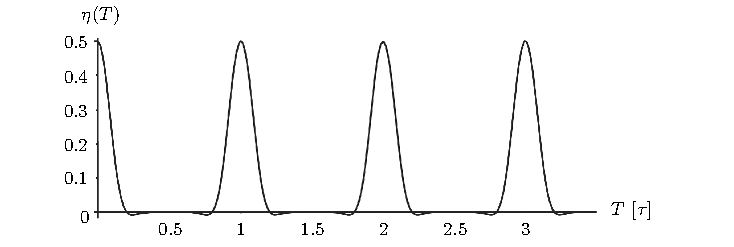
\includegraphics[width=.94\linewidth]{figures/ch06_fig05.pdf}
\caption{Raimond、Brune、Haroche\cite{ref254}が提案した再コヒーレンス実験における、遅延時間$T$に対する二原子相関関数$\eta(T)$の依存性。第二の共振器$\mathrm C_2$、すなわち貯蔵庫によって、$\mathrm C_1$からコヒーレンスが連続的に取り出され、戻される。これが$\mathrm C_1$の猫状態の周期的復活と、最大相関信号$\eta(T)=1/2$の再出現を生む。$T$の単位は、二共振器間でエネルギー、したがって位相情報を交換する特徴的周期$\tau=2\pi/\Omega_{\mathrm C}$である。$\mathrm C_1$の初期場は、平均5個の光子を含むとした。}
\end{figure}

% 原文 p.258
\hypertarget{srcpage:258}{}\label{srcpage:258}
もちろん、現実的な実験設定では、この復活過程は永遠には続かない。共振器$\mathrm C_1$と$\mathrm C_2$は、鏡面での光子損失のような、ほかのデコヒーレンス源や散逸効果を受けるからである。これらの過程は、図6.5の復活ピークの振幅を指数関数的に減衰させることが示されており\cite{ref255}、実際に数個以上のピークを観測できる見込みは低い。それでも、一つの復活ピークの観測だけでも、デコヒーレンスが少なくとも原理的には完全に可逆である事実を、印象的に実験で示すことになる。

\subsectionlink{$\mathrm C_{70}$分子による干渉実験}
本節では、University of ViennaのAnton Zeilingerのグループが行った、一連の実験を述べる。これらは本質的に、よく知られた二重スリット実験を高度に改良したものである。しかしここでは、光や電子のような微視的実体の代わりに、重い分子の干渉模様を観測する。これらの実験が注目すべきなのは、二つの理由による。第一に、通常なら明らかに「物質」の分類に入る物体の、量子的な「波動性」を示す。第二に、デコヒーレンスの連続的作用が、これらの物体から「量子性」を徐々に奪い、経験するおなじみの古典的物体へ変える様子を直接示す。詳しく述べる前に、先行する実験、すなわち単一電子で行われた二重スリット実験を、まず数段落で概説しよう。

\subsubsectionlink{電子による二重スリット実験}
2002年、Physics Worldの読者に、史上「最も美しい物理実験」を選ぶよう求めたところ、一位になったのは、単一電子による二重スリット実験\cite{ref256}だった。Feynmanは、二重スリット実験は「その中に量子力学の核心があり、実際、それは理論の唯一の謎を含む」現象であると述べたことで有名である\cite{ref257}。確かに、量子力学の奇妙な特徴を、これほど単純かつ完全に体現する、ほかの実験を想像するのは難しい。

興味深いことに、電子が二重スリットを通るという元の形でこの実験が実際に行われたのは、1961年、University of TübingenのGottfried Möllenstedtの学生、Claus Jönsson\cite{ref258,ref259}によってであった。Möllenstedtは、それ以前に、電子ビプリズムという別の装置、本質的には電子ビームを二分する非常に細い線を使い、電子の干渉を実験的に示していた。この方法は、19世紀初頭に英国の科学者Thomas Youngが、日光のビームを分け、光が波動的な強め合い・弱め合いの干渉効果を示すことを実証した実験\cite{ref260}で使った、紙片に似ている。
% 原文 p.259
\hypertarget{srcpage:259}{}\label{srcpage:259}
さらに意外かもしれないが、装置内に常に単一電子しかないことを保証した実験は、1989年になって初めて、HitachiのAkira Tonomuraたちが、Möllenstedtと同じく電子ビプリズムを用いて行った\cite{ref261}。得られた干渉模様を図6.6に示す。この実験は、干渉縞が電子間の相互作用で生じるのではなく、個々の電子の波動性によることを示し、量子力学の「謎」を明瞭に反映する。電子ビプリズム干渉計のデコヒーレンスは、最近SonnentagとHasselbach\cite{ref262}が調べた。彼らは、電子と、巨視的で散逸的な電子気体・フォノン気体環境とのCoulomb相互作用によって、干渉模様の可視度が減衰する様子を研究した。

\subsubsectionlink{実験配置}
重い分子の波動性を示すために、Zeilingerのグループが用いた実験配置を概説しよう。Markus Arndtたち\cite{ref263}が1999年のNature論文で報告した最初の実験では、その形から「バッキーボール」と呼ばれることの多い、$\mathrm C_{60}$分子が使われた（図6.7参照）。その後、Zeilingerのグループが2002年の論文\cite{ref264}で初めて結果を報告した実験は、さらに大きな、細長いバッキーボール形の$\mathrm C_{70}$分子と、異なる実験配置\cite{ref264,ref265,ref266,ref267}を用いて行われた。以下では、この後の一連の実験に基づいて論じる。
